\documentclass[tikz,border=10pt]{standalone}
\usepackage{amsmath,amssymb}
\usepackage{tikz}
\usetikzlibrary{arrows.meta,calc,decorations.pathreplacing,patterns,shapes.geometric,positioning,shadings,plotmarks}

\begin{document}
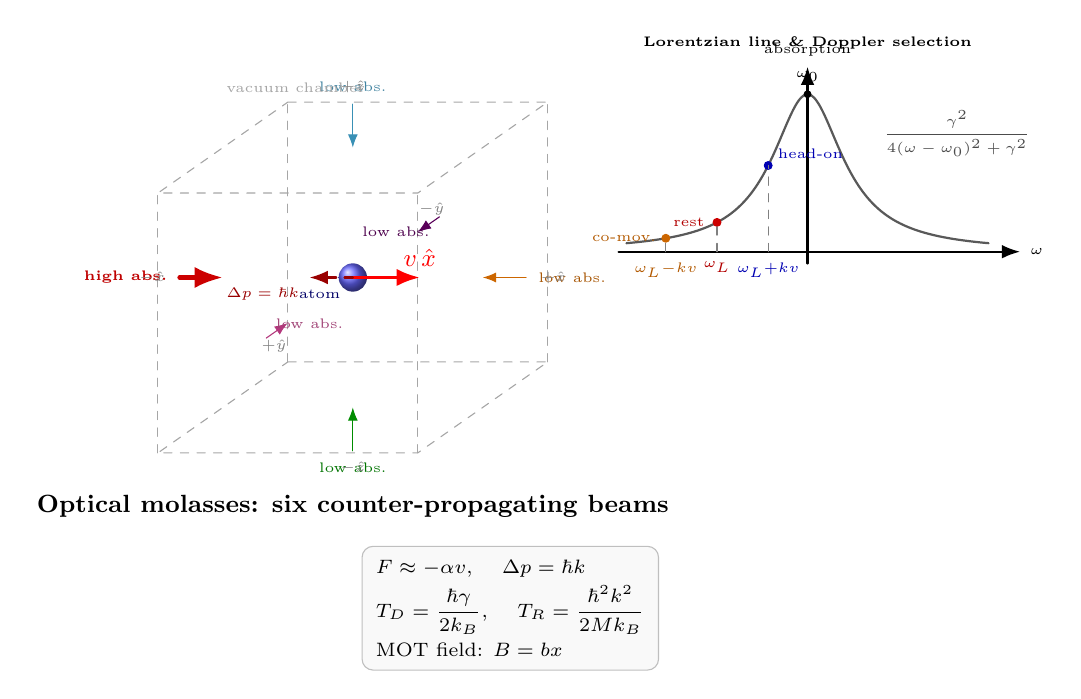
\begin{tikzpicture}[>=Latex, line cap=round, line join=round, font=\footnotesize]

% ========================================================
% Main: 3D optical molasses with six counter-propagating beams
% ========================================================

% Projected axis unit vectors (isometric-ish)
\pgfmathsetmacro{\ax}{1.0}     % +x projected x
\pgfmathsetmacro{\ay}{0.0}     % +x projected y
\pgfmathsetmacro{\bx}{-0.50}   % +y projected (depth into page)
\pgfmathsetmacro{\by}{-0.35}
\pgfmathsetmacro{\cx}{0.0}     % +z projected (up)
\pgfmathsetmacro{\cy}{1.0}

% Cube (vacuum chamber) size L
\pgfmathsetmacro{\L}{3.3}

% Cube corners
\coordinate (O)   at (0,0);
\coordinate (Xp)  at (\L*\ax, \L*\ay);
\coordinate (Yp)  at (\L*\bx, \L*\by);
\coordinate (Zp)  at (\L*\cx, \L*\cy);
\coordinate (XY)  at ($(Xp)+(\L*\bx,\L*\by)$);
\coordinate (XZ)  at ($(Xp)+(\L*\cx,\L*\cy)$);
\coordinate (YZ)  at ($(Yp)+(\L*\cx,\L*\cy)$);
\coordinate (XYZ) at ($(XY)+(\L*\cx,\L*\cy)$);

% Draw dashed cube (vacuum chamber)
\draw[dashed, gray!70, thin]
  (O)--(Xp)--(XY)--(Yp)--cycle;
\draw[dashed, gray!70, thin]
  (Zp)--(XZ)--(XYZ)--(YZ)--cycle;
\draw[dashed, gray!70, thin]
  (O)--(Zp) (Xp)--(XZ) (Yp)--(YZ) (XY)--(XYZ);

% Cube center
\coordinate (C) at ($(O)!0.5!(XYZ)$);

% Face centers (beam endpoints at the faces)
\coordinate (Fxp) at ($(C)+(0.5*\L*\ax,0.5*\L*\ay)$);
\coordinate (Fxm) at ($(C)-(0.5*\L*\ax,0.5*\L*\ay)$);
\coordinate (Fyp) at ($(C)+(0.5*\L*\bx,0.5*\L*\by)$);
\coordinate (Fym) at ($(C)-(0.5*\L*\bx,0.5*\L*\by)$);
\coordinate (Fzp) at ($(C)+(0.5*\L*\cx,0.5*\L*\cy)$);
\coordinate (Fzm) at ($(C)-(0.5*\L*\cx,0.5*\L*\cy)$);

% Extend beam start points slightly outside the cube
\coordinate (Bxp) at ($(Fxp)+(0.55*\ax,0.55*\ay)$);
\coordinate (Bxm) at ($(Fxm)-(0.55*\ax,0.55*\ay)$);
\coordinate (Byp) at ($(Fyp)+(0.55*\bx,0.55*\by)$);
\coordinate (Bym) at ($(Fym)-(0.55*\bx,0.55*\by)$);
\coordinate (Bzp) at ($(Fzp)+(0.55*\cx,0.55*\cy)$);
\coordinate (Bzm) at ($(Fzm)-(0.55*\cx,0.55*\cy)$);

% Five weak beams (thin)
\draw[->, thin, orange!80!black]  (Bxp) -- (Fxp);
\draw[->, thin, magenta!70!black] (Byp) -- (Fyp);
\draw[->, thin, violet!70!black]  (Bym) -- (Fym);
\draw[->, thin, cyan!70!black]    (Bzp) -- (Fzp);
\draw[->, thin, green!55!black]   (Bzm) -- (Fzm);

% Strong beam from -x (counter to v): thick and dark
\draw[->, ultra thick, red!80!black] (Bxm) -- (Fxm);

% Beam labels
\node[orange!65!black,  right=1pt of Bxp]                       {\tiny low abs.};
\node[magenta!60!black, above right=0pt and 0pt of Byp]         {\tiny low abs.};
\node[violet!60!black,  below left=0pt and 0pt of Bym]          {\tiny low abs.};
\node[cyan!60!black,    above=1pt of Bzp]                       {\tiny low abs.};
\node[green!45!black,   below=1pt of Bzm]                       {\tiny low abs.};
\node[red!75!black,     left=1pt of Bxm, align=right]           {\tiny\textbf{high abs.}};

% Axis tick labels
\node[gray, font=\tiny] at ($(Bxp)+(0.35,0.0)$)   {$+\hat{x}$};
\node[gray, font=\tiny] at ($(Bxm)+(-0.35,0.0)$)  {$-\hat{x}$};
\node[gray, font=\tiny] at ($(Byp)+(0.10,-0.10)$) {$+\hat{y}$};
\node[gray, font=\tiny] at ($(Bym)+(-0.10,0.10)$) {$-\hat{y}$};
\node[gray, font=\tiny] at ($(Bzp)+(0.00,0.22)$)  {$+\hat{z}$};
\node[gray, font=\tiny] at ($(Bzm)+(0.00,-0.22)$) {$-\hat{z}$};

% Vacuum chamber label
\node[gray!70, font=\tiny] at ($(Zp)+(0.10,0.18)$) {vacuum chamber};

% Central atom (blue ball with shading)
\shade[ball color=blue!60] (C) circle (0.18);
\node[blue!40!black, font=\tiny, below left=1pt and 1pt of C] {atom};

% Velocity vector v in +x direction (bright red, collinear with -x beam axis)
\coordinate (Vend) at ($(C)+(0.85*\ax,0.85*\ay)$);
\draw[->, very thick, red] (C) -- (Vend) node[above, font=\small, red] {$v\,\hat{x}$};

% Recoil momentum kick from -x absorption: -hbar k xhat at atom
\coordinate (Dpend) at ($(C)-(0.55*\ax,0.55*\ay)$);
\draw[->, thick, red!60!black, dashed] (C) -- (Dpend)
  node[below left, font=\tiny] {$\Delta p=\hbar k$};

% Main title
\node[font=\small\bfseries] at ($(C)+(0,-2.9)$) {Optical molasses: six counter-propagating beams};

% ========================================================
% Inset: Lorentzian resonance curve (top-right)
% ========================================================
\begin{scope}[xshift=6.6cm, yshift=1.4cm]

  % Axes
  \draw[->, thick] (-2.4,0) -- (2.7,0) node[right, font=\tiny] {$\omega$};
  \draw[->, thick] (0,-0.15) -- (0,2.35) node[above, font=\tiny] {absorption};

  % Lorentzian curve (peak at omega_0 = 0, half-width 0.55)
  \draw[thick, gray!70!black, smooth, samples=140, domain=-2.3:2.3]
    plot (\x, {2.0/(1+((\x)/0.55)^2)});

  % omega_0 peak marker
  \filldraw[black] (0,2.0) circle (1.2pt);
  \node[font=\tiny, above=1pt] at (0,2.0) {$\omega_0$};

  % Laser frequency omega_L (red-detuned)
  \pgfmathsetmacro{\wLx}{-1.15}
  \pgfmathsetmacro{\wLy}{2.0/(1+((\wLx)/0.55)^2)}
  \filldraw[red!80!black] (\wLx,\wLy) circle (1.4pt);
  \draw[dashed, gray] (\wLx,0) -- (\wLx,\wLy);
  \node[font=\tiny, below=0pt, red!70!black] at (\wLx,0) {$\omega_L$};
  \node[font=\tiny, left=1pt, red!70!black] at (\wLx,\wLy) {rest};

  % omega_L + kv  (head-on: blue-shifted, closer to resonance)
  \pgfmathsetmacro{\wBx}{-0.50}
  \pgfmathsetmacro{\wBy}{2.0/(1+((\wBx)/0.55)^2)}
  \filldraw[blue!70!black] (\wBx,\wBy) circle (1.4pt);
  \draw[dashed, gray] (\wBx,0) -- (\wBx,\wBy);
  \node[font=\tiny, below=0pt, blue!70!black] at (\wBx,-0.02) {$\omega_L{+}kv$};
  \node[font=\tiny, above right=-1pt and 0pt, blue!70!black] at (\wBx,\wBy) {head-on};

  % omega_L - kv  (co-moving: red-shifted, farther from resonance)
  \pgfmathsetmacro{\wRx}{-1.80}
  \pgfmathsetmacro{\wRy}{2.0/(1+((\wRx)/0.55)^2)}
  \filldraw[orange!80!black] (\wRx,\wRy) circle (1.4pt);
  \draw[dashed, gray] (\wRx,0) -- (\wRx,\wRy);
  \node[font=\tiny, below=0pt, orange!70!black] at (\wRx,-0.02) {$\omega_L{-}kv$};
  \node[font=\tiny, left=0pt, orange!70!black] at (\wRx,\wRy) {co-mov.};

  % Lineshape formula
  \node[font=\tiny, gray!60!black, align=center] at (1.9,1.5)
    {$\dfrac{\gamma^2}{4(\omega-\omega_0)^2+\gamma^2}$};

  % Inset title
  \node[font=\tiny\bfseries] at (0,2.65) {Lorentzian line \& Doppler selection};

\end{scope}

% ========================================================
% Formula block (bottom-right)
% ========================================================
\node[draw=gray!50, rounded corners, fill=gray!5,
      inner sep=5pt, align=left, font=\scriptsize]
  at ($(C)+(2.0,-4.2)$)
  {%
    $F\approx -\alpha v$, \quad
    $\Delta p=\hbar k$ \\[2pt]
    $T_D=\dfrac{\hbar\gamma}{2k_B}$, \quad
    $T_R=\dfrac{\hbar^2 k^2}{2Mk_B}$ \\[2pt]
    MOT field: $B=bx$
  };

\end{tikzpicture}
\end{document}
